%!TEX root = ../main.tex

\RequirePackage{bibentry}
\makeatletter\let\saved@bibitem\@bibitem\makeatother

\documentclass{beamer}
\makeatletter\let\@bibitem\saved@bibitem\makeatother

\renewcommand{\baselinestretch}{1.2}\normalsize
\usetheme{default}
\setbeamertemplate{navigation symbols}{}
\setbeamertemplate{footline}[frame number]

\usepackage{verbatim}
\usepackage{etex}


% BIBLIOGRAPHY APACITE
\usepackage[apaciteclassic]{apacite}
\usepackage{notoccite}
\usepackage{bibentry}
\usepackage{pdfpages}


% MATHEMATICS AND FONTS
\DeclareMathOperator*{\argmin}{arg\,min}
\DeclareMathOperator*{\argmax}{arg\,max}

\renewcommand{\vec}[1]{\mathbf{#1}}

\usepackage{amsfonts}
\usepackage{amsmath}
\usepackage{amssymb}
\usepackage{bbm}
\usepackage{algpseudocode}
\usepackage{setspace}

\usepackage{arev}
\usepackage[latin1]{inputenc}
\usepackage[T1]{fontenc}


% GRAPHS
\usepackage{graphicx}
\usepackage{subfig}
\usepackage{caption}
\graphicspath{{material/}}
\usepackage{relsize}
\usepackage{lscape}
\usepackage{fancybox}
\usepackage{epstopdf}


% TABLES AND OTHER ENVIRONMENTS
\usepackage{tabularx}
\usepackage{longtable}
\usepackage{booktabs}
\usepackage{color,colortbl}
\usepackage{threeparttable}

\usepackage{enumerate}

\usepackage{fix-cm}

\usepackage{bookmark}
\usepackage{hyperref}
\hypersetup{colorlinks=true,urlcolor=blue,citecolor=black}


\usepackage{tikz}
\tikzset{
	treenode/.style = {shape=rectangle, rounded corners,
		draw, align=center,
		top color=white, bottom color=blue!20},
	root/.style     = {treenode, font=\Large, bottom color=red!30},
	env/.style      = {treenode, font=\ttfamily\normalsize},
	dummy/.style    = {circle,draw}
}
%\usepackage{cmbright}
\def\newblock{\hskip .11em plus .33em minus .07em}
\newcommand{\bs}{\boldsymbol}
\newcommand{\N}{\mathbb{N}}
\newcommand{\cov}{\mathrm{cov}\thin}
\newcommand{\thin}{\thinspace}
\newcommand{\thick}{\thickspace}
\newcommand{\Lim}[1]{\raisebox{0.5ex}{\scalebox{0.8}{$\displaystyle \lim_{#1}\;$}}}

\newcommand{\vect}[1]{\mathbf{#1}}
\newcommand{\myfrac}[3][0pt]{\genfrac{}{}{}{}{\raisebox{#1}{$#2$}}{\raisebox{-#1}{$#3$}}}
\newcommand{\U}{\mathrm{U}}	%Uniform Distribution
\newcommand{\D}{\mathrm{D}}	%Dirichlet Distribution
\newcommand{\W}{\mathrm{W}}	%Wishart Distribution
\newcommand{\E}{\mathrm{E}}		%Expectation
\newcommand{\Prob}{\mbox{Pr}}		%Expectation
\newcommand{\Iden}{\mathbb{I}}	%Identity Matrix
\newcommand{\Ind}{\mathrm{I}}	%Indicator Function
\newcommand{\Tau}{\mathcal{T}\thin}

\newcommand{\var}{\mathrm{var}\thin}
\newcommand{\plim}{\mathrm{plim}\thin}
\newcommand\indep{\protect\mathpalette{\protect\independenT}{\perp}}
\def\independenT#1#2{\mathrel{\rlap{$#1#2$}\mkern5mu{#1#2}}}
\newcommand{\notindep}{\ensuremath{\perp\!\!\!\!\!\!\diagup\!\!\!\!\!\!\perp}}%

\newcommand{\mc}{\multicolumn}

\newcommand{\ph}{\phantom}
% weitere Optionen:
% secbar: Gliederung im Kopf, nur sections (alternativ zu subsecbar)
% handout: Produktion von Handouts, keine Animationen
\definecolor{darkblue}{rgb}{0,.35,.62}
\definecolor{lightblue}{rgb}{0.8,0.85,1}
\definecolor{lightgrey}{gray}{0.1}	%Farben mischen

%	kbordermatrix options

\makeatletter
\newcommand{\vast}{\bBigg@{4}}
\newcommand{\Vast}{\bBigg@{5}}
\makeatother
\newcommand{\indicator}[1]{\mathbbm{1}{\left\{ {#1} \right\} }}
\newcommand{\indic}{1{\hskip -2.5 pt}\hbox{1} }


\definecolor{lightgrey}{gray}{0.90}	%Farben mischen
\definecolor{grey}{gray}{0.85}
\definecolor{darkgrey}{gray}{0.65}
\definecolor{lightblue}{rgb}{0.8,0.85,1}

\renewcommand{\arraystretch}{1.5}


\usepackage{tikz}
\usetikzlibrary{trees,shapes,arrows,decorations.pathmorphing,backgrounds,positioning,fit,petri}
\renewcommand*{\familydefault}{\sfdefault}

\tikzset{forestyle/.style = {rectangle, thick, minimum width = 5cm, minimum height = 0.5cm, text width = 4.5cm, outer sep = 1mm},
	pre/.style={<-, shorten <=1pt, >=stealth, ultra thick},
	extend/.style={<-,dashed, shorten <=1pt, >=stealth, ultra thick}}
\captionsetup[subfigure]{labelformat=empty}


\newcommand{\beginbackup}{
	\newcounter{framenumbervorappendix}
	\setcounter{framenumbervorappendix}{\value{framenumber}}
}
\newcommand{\backupend}{
	\addtocounter{framenumbervorappendix}{-\value{framenumber}}
	\addtocounter{framenumber}{\value{framenumbervorappendix}}
}


% Begin Full Justification ---------------------------------------------------------

\usepackage{ragged2e}
% \usepackage{etoolbox}
\usepackage{lipsum}
\makeatletter
\renewcommand{\itemize}[1][]{%
	\beamer@ifempty{#1}{}{\def\beamer@defaultospec{#1}}%
	\ifnum \@itemdepth >2\relax\@toodeep\else
	\advance\@itemdepth\@ne
	\beamer@computepref\@itemdepth% sets \beameritemnestingprefix
	\usebeamerfont{itemize/enumerate \beameritemnestingprefix body}%
	\usebeamercolor[fg]{itemize/enumerate \beameritemnestingprefix body}%
	\usebeamertemplate{itemize/enumerate \beameritemnestingprefix body begin}%
	\list
	{\usebeamertemplate{itemize \beameritemnestingprefix item}}
	{\def\makelabel##1{%
			{%
				\hss\llap{{%
						\usebeamerfont*{itemize \beameritemnestingprefix item}%
						\usebeamercolor[fg]{itemize \beameritemnestingprefix item}##1}}%
			}%
		}%
	}
	\fi%
	\beamer@cramped%
	\justifying% NEW
	%\raggedright% ORIGINAL
	\beamer@firstlineitemizeunskip%
}

\justifying

% \apptocmd{\frame}{\justifying}{}{}

\usepackage{array}
\newcolumntype{L}[1]{>{\raggedright\let\newline\\\arraybackslash\hspace{0pt}}m{#1}}
\newcolumntype{C}[1]{>{\centering\let\newline\\\arraybackslash\hspace{0pt}}m{#1}}
\newcolumntype{R}[1]{>{\raggedleft\let\newline\\\arraybackslash\hspace{0pt}}m{#1}}



% End Full Justification ------------------------------------------------------------


%!TEX root = ../main.tex
\title{Estimating Marginal Returns to Education}
\author{Carneiro, P., Heckman, J. J., and Vytlacil, E. J.}

\date{}

\let\otp\titlepage
%\renewcommand{\titlepage}{\otp\addtocounter{framenumber}{-1}}

\begin{document}
\nobibliography*
\maketitle

 \begin{frame}
\begin{quote} This paper estimates marginal returns to college for individuals induced to enroll in college by different marginal policy changes. The recent instrumental variables literature seeks to estimate this parameter, but in general it does so only under strong assumptions that are tested and found wanting. We show how to utilize economic theory and local instrumental variables estimators to estimate the effect of marginal policy changes. Our empirical analysis shows that returns are higher for individuals with values of unobservables that make them more likely to attend college. We contrast our estimates with IV estimates of the return to schooling.
\end{quote}
 \end{frame}


\begin{frame}\begin{center}\begin{figure}[htp]\centering
\scalebox{0.75}{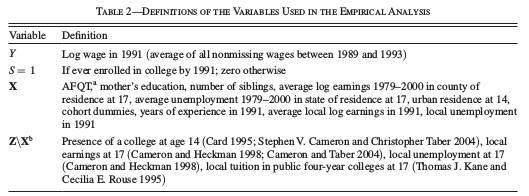
\includegraphics{fig-empirical-specification}}
\end{figure}\end{center}\end{frame}

\begin{frame}\begin{center}\begin{figure}[htp]\centering
\scalebox{0.75}{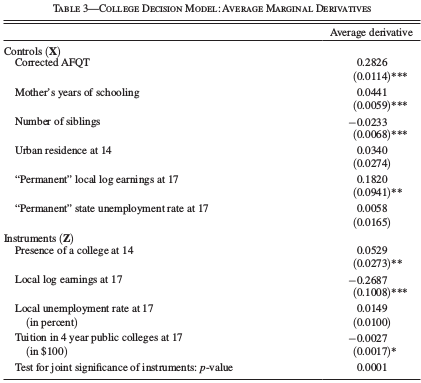
\includegraphics{fig-choice-model}}
\end{figure}\end{center}\end{frame}

\begin{frame}\begin{center}\begin{figure}[htp]\centering
\scalebox{0.75}{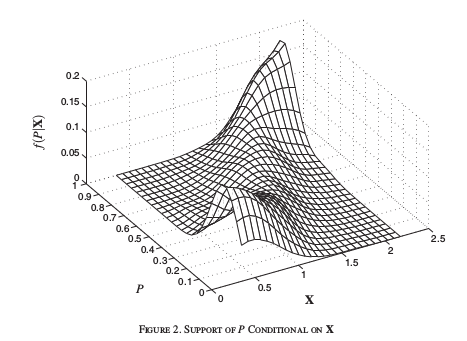
\includegraphics{fig-common-support}}
\end{figure}\end{center}\end{frame}


\begin{frame}\begin{center}\begin{figure}[htp]\centering
\scalebox{0.75}{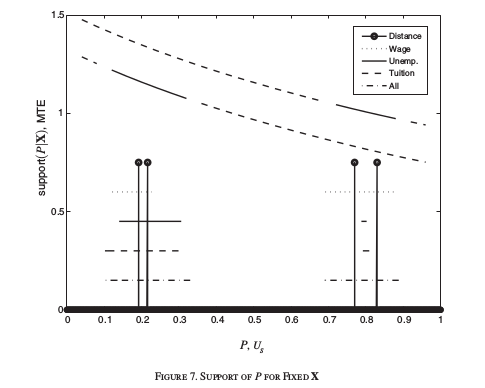
\includegraphics{fig-conditional-support}}
\end{figure}\end{center}\end{frame}

\begin{frame}\begin{center}\begin{figure}[htp]\centering
\scalebox{0.75}{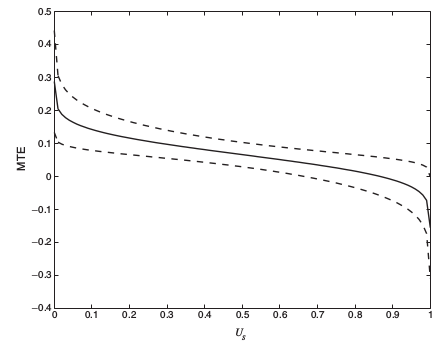
\includegraphics{fig-marginal-benefit-parametric}}
\end{figure}\end{center}\end{frame}

\begin{frame}\begin{center}\begin{figure}[htp]\centering
\scalebox{0.75}{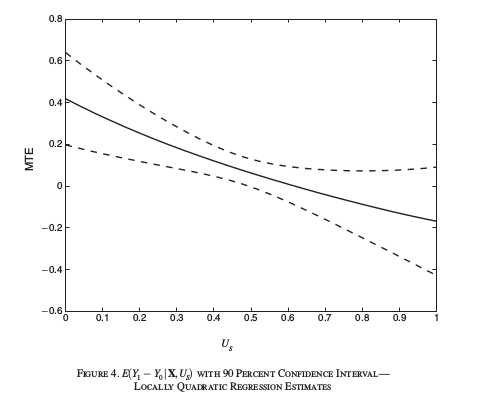
\includegraphics{fig-marginal-benefit-semiparametric}}
\end{figure}\end{center}\end{frame}

\begin{frame}\begin{center}\begin{figure}[htp]\centering
\scalebox{0.75}{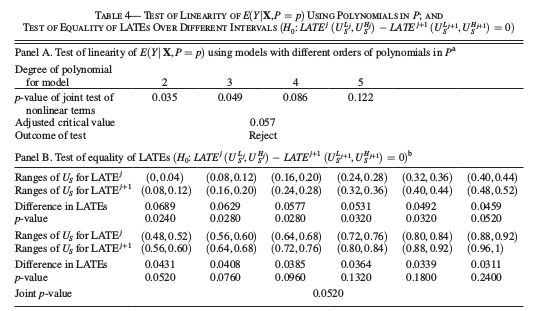
\includegraphics{fig-eh-test}}
\end{figure}\end{center}\end{frame}

\begin{frame}\begin{center}\begin{figure}[htp]\centering
\scalebox{0.75}{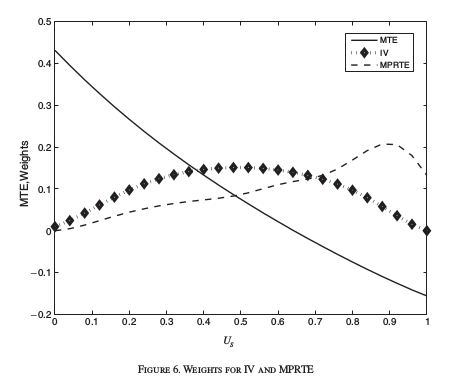
\includegraphics{fig-marginal-weights}}
\end{figure}\end{center}\end{frame}

\begin{frame}\begin{center}\begin{figure}[htp]\centering
\scalebox{0.75}{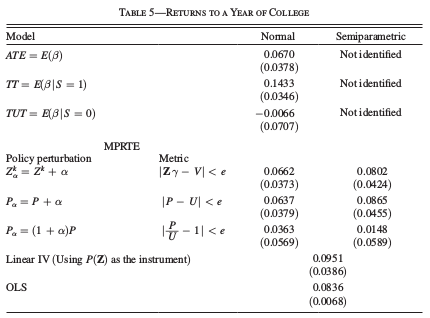
\includegraphics{fig-treatment-parameters}}
\end{figure}\end{center}\end{frame}

%!TEX root = ../main.tex
\beginbackup\appendix
\begin{frame}\begin{center}
\LARGE\textbf{Appendix}
\end{center}\end{frame}

%------------------------------------------------------------------------------
%------------------------------------------------------------------------------
\begin{frame}\begin{center}
\LARGE\textit{References}
\end{center}\end{frame}
%------------------------------------------------------------------------------
%------------------------------------------------------------------------------
\newgeometry{margin=1cm}
\begin{frame}[allowframebreaks]\frametitle{}

\nocite{Carneiro.2011}

\bibliographystyle{apacite}
\bibliography{../../../submodules/bibliography/literature}


\end{frame}

\backupend
\end{document}
\grid
